\documentclass[12pt]{article}
 \usepackage[margin=1in]{geometry}
\usepackage{amsmath,amsthm,amssymb,amsfonts,algorithm,algpseudocode,algorithmicx,xfrac}

\newcommand{\N}{\mathbb{N}}
\newcommand{\Z}{\mathbb{Z}}

\newenvironment{problem}[2][Problem]{\begin{trivlist}
\item[\hskip \labelsep {\bfseries #1}\hskip \labelsep {\bfseries #2.}]}{\end{trivlist}}
\newenvironment{subproblem}[1]{\textbf{(#1)}}{}

\theoremstyle{definition}
\newtheorem{definition}{Definition}[section]

\newtheorem{theorem}{Theorem}[section]
\newtheorem{corollary}{Corollary}[theorem]
\newtheorem{lemma}[theorem]{Lemma}
%If you want to title your bold things something different just make another thing exactly like this but replace "problem" with the name of the thing you want, like theorem or lemma or whatever

\begin{document}

%\renewcommand{\qedsymbol}{\filledbox}
%Good resources for looking up how to do stuff:
%Binary operators: http://www.access2science.com/latex/Binary.html
%General help: http://en.wikibooks.org/wiki/LaTeX/Mathematics
%Or just google stuff

\title{Social Computing - Homework 2}
\author{Howie Benefiel \(phb337\) and Kelsey Sandlin \(kk29746\) }
\maketitle

\begin{problem}{1}
$ $ \newline

\begin{subproblem}{a}

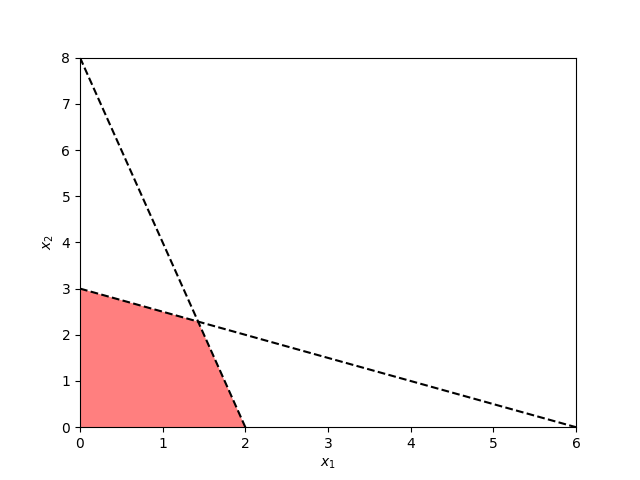
\includegraphics[width=\textwidth]{feasibleq1.png}
\end{subproblem}

\begin{subproblem}{b}
The vertices are $(x_1, x_2)$: $(0, 0), (0, 3), (2, 0), (\sfrac{10}{7}, \sfrac{16}{7})$.
\end{subproblem}

\begin{subproblem}{c}
The optimal value is at $(0, 3)$: 18.
\end{subproblem}

\begin{subproblem}{d}
\begin{equation*}
\begin{array}{ll@{}ll}
\text{minimize}  & 8x_1 + 6x_2 \\
\text{subject to}& 4x_1+x_2 \geq 2\\
                 & x_1 + 2x_2 \geq 6\\
                 & x_1, x_2 \geq 0

\end{array}
\end{equation*}
\end{subproblem}

\begin{subproblem}{e}
$ $ \newline
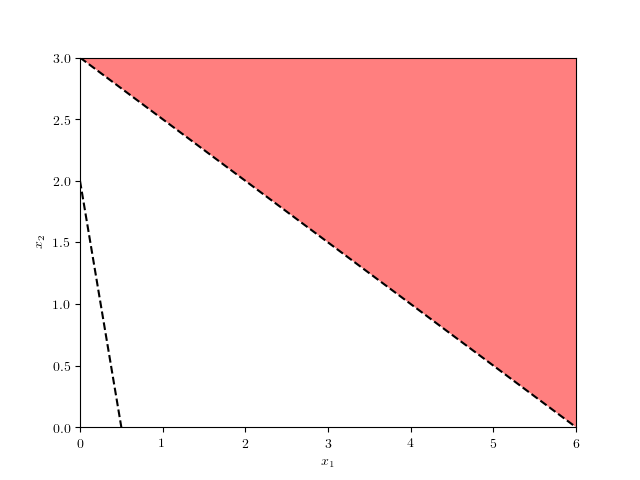
\includegraphics[width=\textwidth]{feasibledual.png}
\end{subproblem}

\begin{subproblem}{f}
The optimal value is at $(0, 3)$: 18.
\end{subproblem}

\end{problem}



\begin{problem}{2}
$ $ \newline

Let $ P=\{(m, w), \dots \} $ be a male-optimal pairing output by the Gale-Shapley algorithm.
We want to show that $ P $ is woman-pessimal by showing that any other pairing, $ P^{'} $ , that is more woman-pessimal that $ P $ is also unstable.

Let $ P= \{ (m^{'}, w), (m,w^{'}), \dots \} $ be a matching that is more woman-pessimal than $ P $ .
This means that $ w $ must prefer m to her $ P^{'} $ pairing $ m^{'} $.
Since our original pairing $ P $ is man-optimal, we know $ m $ must prefer $ w $ to $ w^{'} $ .
Since $ w $ prefers $ m $ to her $ P^{'} $ partner $ m^{'} $ and $ m $ prefers $ w $ to her $ P^{'} $ partner $ w $ , the pairing $ P^{'} $ is unstable.

Since $ P^{'} $ is unstable, we have show that $ P $ is the most woman-pessimal stable marriage.

\end{problem}



\begin{problem}{3}

\begin{subproblem}{a}
The proposed algorithm is based off the following fact.
There must be a stable marriage which exists where the following are true:
First, the marriage $ (m, w) $ is only stable if all the women which $ m $ prefers over $ w $ are paired with men who $ w $ prefers over $ m $ .
And the inverse must also be true, all the men who $ w $ prefers over $ m $ must be paired with women who $ m $ prefers to $ w $ .

First, we remove $ m $ and $ w $ from each of the remaining preference lists.
Then when running Gale-Shapley algorithm, if $ rank([w][m^{'}]) > rank([w][m])$ where $ w $ is the woman in the stable pair to be tested, $ m $ is the man in the stable pair to be tested and $ m^{'} $ is the currently choosing man,
then we have $ m^{'} $ choose a woman who $ m $ prefers to $ w $ who he has not previously proposed to.
If at any point a man does not have a valid choice given that rule, then there is no stable matching.
If the program terminates with a perfect matching, then there is a stable matching between $ (m, w) $.
\end{subproblem}

\begin{subproblem}{b}
I would give the output of my algorithm for part \textbf{a}.
\end{subproblem}

\begin{subproblem}{c}
I would give the stable matching where $ (m, w) $ had been removed and the facts from part \textbf{a} were true:
The women which $ m $ prefers over $ w $ are paired with men who $ w $ prefers over $ m $ .
And all the men who $ w $ prefers over $ m $ must be paired with women who $ m $ prefers to $ w $ .
\end{subproblem}

\end{problem}




\end{document}
